% #############################################################################
% This is Chapter 2
% !TEX root = ../main.tex
% #############################################################################
% Change the Name of the Chapter i the following line
\fancychapter{Background}
% The following line allows to ref this chapter
\label{chap:back}

This chapter introduces the fundamental concepts of \glsxtrfull{IR}, while \glsxtrfull{NLP} will be addressed in the following state-of-the-art chapter. \glsxtrfull{IR} has evolved from lexical to semantic search, and understanding these approaches is essential to contextualize how \glsxtrfull{NLP} later enables agents to reason over retrieved information to provide more intelligent responses. The following section presents these \glsxtrfull{IR} approaches and the optimizations that have evolved from them.
\section{Background on Transformers} 
\label{sec:transformer}
\subsection{The Transition from Sequential to Attention-Based Models}  
Traditional sequence transduction models, such as \glsxtrfull{RNN} and its variants (e.g., \glsxtrfull{LSTM} \cite{hochreiter1997lstm} and \glsxtrfull{GRU} \cite{cho2014gru}), were widely used in tasks such as machine translation and language modeling. Although effective, these models relied on sequential calculations, which limited their parallelization and computational efficiency in long sequences \cite{vaswani2017attention}.

In 2017, Vaswani et al. introduced the Transformer architecture, marking a significant change from these sequential models. Transformer relies exclusively on attention mechanisms, specifically self-attention, to model dependencies between input and output sequences. By removing recursive and convolutional operations, Transformer achieves faster training times and superior performance in generative operations \cite{vaswani2017attention}.

\begin{figure}[H]
    \centering
    % First image
    \centering
    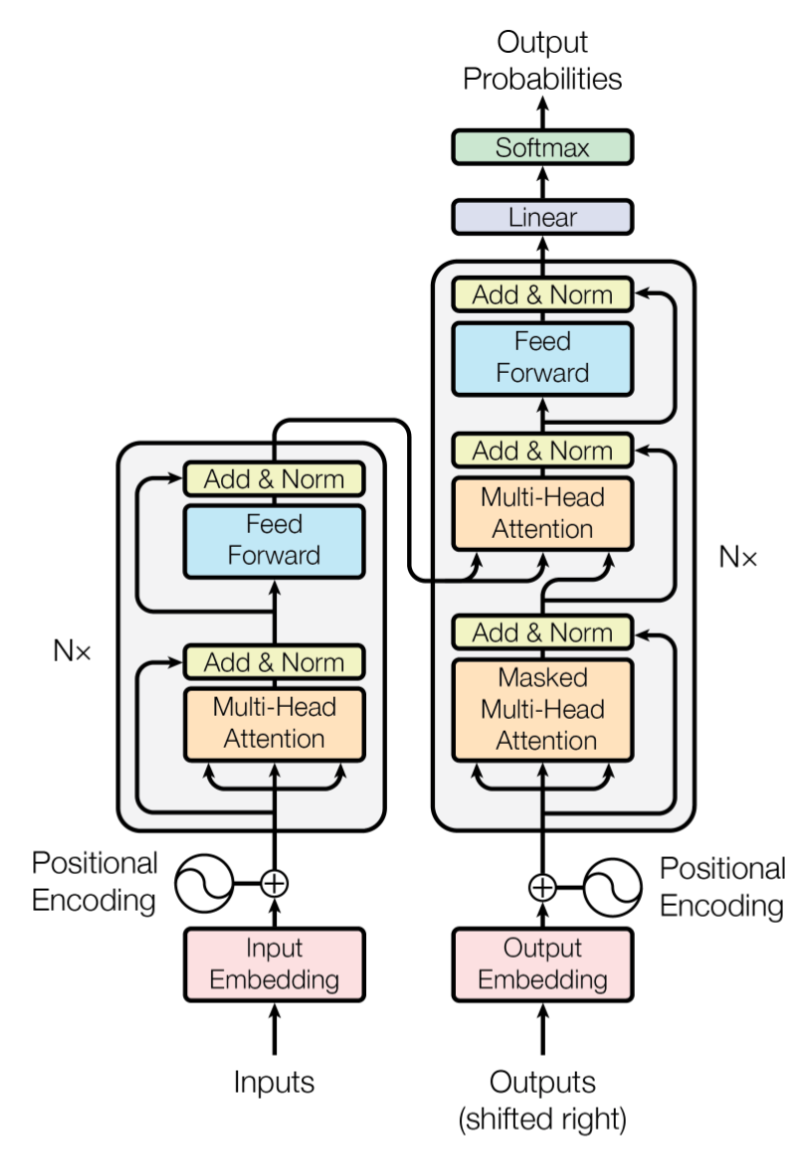
\includegraphics[width=0.45\linewidth]{Images/Transformer_architecture3.png}
    \caption{Transformer Architecture from\cite{vaswani2017attention}}
    \label{fig:Tranformer}
\end{figure}
\subsection{Main Innovations in Transformer Architecture}  
\begin{itemize}
    \item \textbf{Embeddings}: Learned embeddings convert input and output tokens to vectors of dimension $d$ depending on the dimension of the model. Tokens are discrete symbols of words or subwords.
    
    \item \textbf{Positional Coding}:  
    Transformers do not need recurrence nor convolution, instead some information about relative or absolute position of the tokens is injected in the sequences. This is the positional encodings added to the input embeddings. \cite{vaswani2017attention}.  
    \item  \textbf{Scaled Dot-Product Attention} \ref{eq:Attention}: Is an attention function \ref{eq:Attention} that maps a query and a set of key-value pairs to an output.
    \begin{equation}
        \label{eq:Attention}
        \text{Attention}(Q,K,V) = softmax(\frac{QK^T}{\sqrt{d_k}})V 
    \end{equation} 
    \begin{itemize}
        \item Q is a set of keys packed together into a matrix.
        \item K and V are also matrices packed together of keys and values, respectively
    \end{itemize}
    \item \textbf{Multi-Head Attention}:  Queries, keys and values are linearly projected $h$ different times with different learned linear projections\ref{eq:MultiHead}. The Multi-head attention allows the model to jointly attend to information from different representation subspaces at different positions. \textbf{Masked Multi-Head Attention} masks future positions in the sequence during the decoding process\cite{vaswani2017attention}.
    \begin{equation}
        \label{eq:MultiHead}
        \text{MultiHead}(Q,K,V) = \text{Concat}(head_1, ..., head_h)W^O  
    \end{equation}
    \begin{itemize}
        \item $head_i = \text{Attention}(QW_i^Q, KW_i^K,VW_i^V)$
    \end{itemize}
    \item \textbf{Feed-Forward}:  A Position-Wise Feed-Forward Network (FFN) \ref{eq:FNN} is a fully connected neural network designed to independently process each position in the sequence.  While FNN \ref{eq:FNN} operates identically at all positions, the parameters vary between layers. The dimension of the inner-layer has a larger dimension than the model's dimension to increase its capacity to learn complex transformation\cite{vaswani2017attention}.
    \begin{equation}
        \label{eq:FNN}
        \text{FNN}(x) = \max(0,xW_1+b_1)W_2+b_2
    \end{equation}
\end{itemize}




\subsection{Performance and Impact}  
The Transformer architecture achieved top results in machine translation tasks, such as on the WMT 2014 English-German and English-French datasets, with significantly shorter training times compared to previous models. For example, the model achieved a BLEU score of 28.4 on English-to-German translation, outperforming previous architectures by more than 2 BLEU points \cite{vaswani2017attention}.  
The Transformer architecture has had a transformative impact on \glsxtrfull{NLP} . It serves as the basis for \glsxtrfull{LLM} models such as BERT, GPT and others, which are based on the core principles of self-attention and scalability.

\section{Large Language Models (LLMs)}
\label{sec:llm}
Are transformer \ref{sec:transformer} based models trained on massive text corpora to generate natural language with high semantic accuracy \cite{bertpretrainingdeepbidirectional}.
Summarization and reasoning are key capabilities of \glsxtrfull{AAI} systems, which must distill context, interpret complex instructions, and generate coherent responses.
While open-source models such as LLaMA, Mistral, and Falcon (available via Hugging Face) offer valuable baseline options, this thesis primarily utilizes the OpenAI API. Compared to hosting open-source models on local servers, OpenAI’s approach is cheaper, higher-performing, and more scalable, since it removes infrastructure costs while providing access to cutting-edge systems like GPT-4o and GPT-4o-mini.

Strong empirical evidence supports this choice:
\begin{itemize}
  \item On Brazilian Portuguese grammatical error correction tasks, GPT-4 outperformed alternatives in recall, demonstrating improved handling of Portuguese grammar \cite{arxiv2306.15788}.
  \item On the Brazilian ENEM entrance exam, GPT-4 with Chain-of-Thought prompting achieved 87\% accuracy, surpassing GPT-3.5 by approximately 11 points \cite{arxiv2303.17003}.
  \item On the Portuguese National Medical Residency Access Examination, GPT-4o outperformed open-source model LLaMA 3.1 by 7–11\% across multiple medical domains \cite{pmc12166901}.
  \item In another Portuguese medical benchmark, ChatGPT-4o significantly outperformed ChatGPT-3.5 (median score: 127 vs.\ 106) and ranked in the top 1\% of human candidates \cite{amp2025gpt4o}.
\end{itemize}

Given these performance advantages, even performing well in the Portuguese language, along with cost-effectiveness and scalability, OpenAI \glsxtrfull{LLM}s are adopted in this thesis as the principal agents for reasoning and summarization.


\section{\glsxtrfull{RAG}}
\label{sec:rag}

Retrieval-Augmented Generation (\glsxtrfull{RAG}) is a framework designed to improve performance on knowledge-intensive \glsxtrfull{NLP} tasks. It combines \textit{parametric knowledge}, implicitly stored in the parameters of a pre-trained \glsxtrfull{LLM}, with \textit{non-parametric knowledge}, retrieved from external sources such as document collections or databases. Instead of relying solely on the static internal knowledge of the model, RAG enhances generation with dynamically retrieved and contextually relevant information.

\subsection{Parametric and Non-Parametric Knowledge}
Traditional \glsxtrfullpl{LLM} encode knowledge implicitly in their parameters, known as parametric knowledge. Although powerful, this knowledge is static, cannot be updated without retraining, and may become outdated.  
\glsxtrfull{RAG} mitigates this limitation by introducing a retrieval component that accesses external, explicit, and up-to-date information, known as non-parametric knowledge. So to use AI for semantic search, it is essential to use \glsxtrfull{RAG} for up to date information.

\subsection{The Three Stages of RAG}
A typical RAG pipeline operates in three sequential stages:
\begin{enumerate}
    \item \textbf{Retrieval:} Given an input query, the system searches an external knowledge base (e.g., a vector database) to retrieve the most relevant documents or passages.  
    \item \textbf{Augmentation:} The retrieved documents/chunks of text are then combined with the query to form an enriched prompt, providing the \glsxtrfull{LLM} with additional context.  
    \item \textbf{Generation:} The \glsxtrfull{LLM} conditions its output on both the query and the retrieved context, producing responses from known sources. 
\end{enumerate}

\subsection{Sparse Retrieval Methods}
The retrieval stage can be implemented in multiple ways. Traditional approaches rely on \textbf{sparse representations}, where documents are represented as bags of words or weighted keyword vectors. Well-known methods include:
\begin{itemize}
    \item \textbf{TF-IDF:} retrieves documents based on term frequency and inverse document frequency weighting.  
    \item \textbf{BM25:} an advancement over TF-IDF, incorporating term saturation and document length normalization for more robust scoring.  
\end{itemize}

Later methods extend retrieval to dense vector representations (see Section~\ref{sec:vector-databases}), enabling semantic similarity search beyond exact keyword matching.

\subsubsection{TF-IDF (Term Frequency-Inverse Document Frequency)}
TF-IDF is a foundational term-weighting and ranking scheme in information retrieval systems \cite{tf-idf}. Its primary purpose is to measure how important a term is to a particular document within a large collection of documents. While frequency counts can highlight terms that often appear, they do not account for how common or rare those terms are across the entire dataset. TF-IDF addresses this by diminishing the weight of terms that occur frequently across many documents and increasing the weight of terms that appear in fewer documents (more distinctive terms).
The \glsxtrfull{TF} measures how often a term \textit{t} appears in a single document \textit{d}. 
\begin{equation}
    \label{eq:tf} 
    \text{TF}(t,d)=f_{t,d}
\end{equation}
For longer documents a normalization is used a such:
\begin{equation}
    \label{eq:tf(t,d)}
    \text{TF}(t,d) = \frac{f_{t,d}}{\sum_{t'}f_{t',d}}
\end{equation}
The inverse document frequency (IDF) measures how common a term is across the entire collection of documents. If a term appears in many documents, it is less useful for distinguishing those documents. A higher IDF means a term appears in fewer documents, indicating its uniqueness. \textit{N} is the total number of documents in the collection, and $n_t$ is the number of documents in which the term appears. \textit{IDF} is defined as:
\begin{equation}
    \label{eq:idftf}
    \text{IDF}(t)=\log\frac{N}{n_t}
\end{equation}
TF-IDF is then the combination of both TF and IDF
\begin{equation}
    \label{eq:tfidf}
    \text{TF-IDF}(t,d) = f_{t,d} \times \log\left(\frac{N}{n_t}\right)
\end{equation}
The uniqueness of the TF-IDF approach in retrieval is how it combines a local component (frequency in the current document) and a global component (frequency across the entire collection). TF-IDF has the advantage of being straightforward, interpretable, and computationally efficient.

\subsubsection{BM25 (Okapi BM25)}
The okapi system first introduced in\cite{Bm25foundation} which then culminated to BM25. The BM25(short for "Best Match 25") is a probabilistic information retrieval model. This information retrieval model improves upon TF-IDF by using a probabilistic basis rather than a purely heuristic bases, and by introducing parameters to control term frequency by saturation, and document length normalization.
The BM25 formulas is similar to the TF-IDF as it uses a more sophisticated formulation of the IDF component found in TF-IDF this one is more stable and empirically effective. The IDF component per term \textit{t} is computed as:
\begin{equation}
    \label{eq:idfbm25}
    \text{IDF}(t) = \log \frac{N-n_t+0.5}{n_t+0.5}
\end{equation}
where N is the total number of documents in the collection and $n_t$ is the number of documents containing term \textit{t}.

BM25 formula to score a document from a query( a number of terms) looks like \cite{bm25}:
\begin{equation}
    \label{eq:bm25}
    \textit{BM25}(d,q) = \sum_{t \in q} IDF(t) \cdot \frac{(k_1+1)\cdot f_{t,d}}{f_{t,d}+k_1(1-b+b \cdot \frac{|d|}{avgdl})}
\end{equation}
where:
\begin{itemize}
\item $d$ is a given document.
\item $q$ a user's query, consisting of t terms.
\item $|d|$ is the length of a document in terms of the number of tokens.
\item $dl$ is document length $:=\sum_{i \in V}{tf}_i$
\item $avgdl$ is average document length across the entire collection
\item $k_1$ and $b$ are tuning parameters:
\begin{itemize}
    \item $k_1$ controls  the saturation of \glsxtrfull{TF}, by preventing over-emphasis on very frequent terms.
    \item $b$ controls the amount $dl$ is normalized. If $b = 1$, the normalization is directly proportional to how much longer( or shorter) the document ($|d|$) is compared to average document length ($avgdl$). if $b=0$, no document length ($dl$) is applied.
\end{itemize}
\end{itemize}

\subsection{Vector-based Retrieval Methods}

Retrieval of a relevant document from a large collection, based on a user query, was traditionally implemented using TF-IDF or BM25 \cite{bm25}. These are sparse vector space models that match keywords efficiently via an inverted index. Under such methods, both queries and documents are represented as high-dimensional, sparse vectors with term-based weighting. While these models are often effective for keyword-based matches, they struggle when queries and relevant documents use synonyms or paraphrases that do not share surface-level terms.

Recent advancements in \glsxtrfull{LLM}, particularly transformer-based models like BERT \cite{bertpretrainingdeepbidirectional}, have led to dense retrieval systems. In dense retrieval, queries and documents are represented as low-dimensional vectors that better capture semantic similarity. However, dense methods often require large training datasets (i.e., labeled question–passage pairs) to surpass classical methods such as TF-IDF/BM25. Modern pre-trained language models help mitigate this requirement by providing robust initial embeddings that can be fine-tuned on relatively smaller sets of question–context examples. This opens the door for dense retrieval methods to outperform traditional sparse approaches in many open-domain QA tasks.
\subsubsection{Dense Passage Retrieval (DPR)}
\label{par:dpr}
Dense Passage Retrieval (DPR), introduced by Karpukhin et al.~\cite{densepassageretrievalopendomainkarpukhin2020}, is a \textit{dense retrieval} method designed specifically for \textit{open-domain question answering}. Unlike conventional approaches that rely on \textit{purely lexical} matches (e.g., TF-IDF and BM25), DPR employs BERT-based encoders to map questions and passages into a shared, dense embedding space, enabling \textit{semantic} rather than strictly \textit{keyword-based} retrieval. By leveraging modern \glsxtrfull{LLM} such as BERT~\cite{bertpretrainingdeepbidirectional} and LLaMA, which come with strong pre-trained representations, DPR can be fine-tuned with comparatively fewer labeled samples. This allows the system to capture semantic relationships between questions and passages, thereby mitigating the shortcomings of traditional methods that rely solely on term overlap.

The DPR architecture is based on a dual-encoder architecture~\cite{dualencoderarchitecture}. Specifically, in Karpukhin et al.'s formulation~\cite{densepassageretrievalopendomainkarpukhin2020}, both encoders are initialized from the same pre-trained BERT model but are then fine-tuned separately for their respective tasks. A Question Encoder \(E_Q\) takes a question as input and produces a single vector embedding \(q_i\), while a Passage Encoder \(E_P\) processes a passage to produce a single vector embedding \(p_j\). Once encoded, each question and passage becomes a fixed-dimensional vector (e.g., 768 dimensions). To measure the similarity between a question \((q)\) and a passage \((p)\), the dot product of their embeddings is computed:
\begin{equation}
    \label{eq:dot_sim}
    \text{similarity}(q, p) = E_Q(q)^T \, E_P(p).
\end{equation}

%For very large document collections (e.g., a full Wikipedia dump), a dense vector index like \glsxtrfull{FAISS} \cite{DOUZE2024FAISS} is typically used to support efficient similarity searches. \glsxtrfull{FAISS} is a specialized library designed for rapid similarity search and clustering of dense vectors, enabling the system to scale to billions of embeddings. Concretely, DPR encodes all passages offline with \(E_P\), storing the resulting passage embeddings \((p_j)\) in the \glsxtrfull{FAISS} index. This offline procedure ensures that the more computationally intensive step—embedding the entire corpus—happens only when the vector database needs to be updated.
%


\section{Sentence Transformers}
\label{sec:Sentence-Transformers}
Sentence Transformers are BERT-based encoder models designed to generate dense vector representations (embeddings) of entire sentences or passages. 
They were introduced in 2019 \cite{reimers2019sentencebertsentenceembeddingsusing} as an adaptation of the BERT architecture, which was originally built for token-level classification tasks.

With the use of Siamese and Triplet network structures on top of BERT, SBERT modifies the architecture to operate at the sentence level. Instead of encoding a pair of sentences jointly, as in the cross-encoder setup of standard BERT, SBERT processes each sentence independently with a shared BERT encoder. This produces fixed-size embeddings that can later be compared directly using cosine similarity or other distance metrics, making large-scale similarity search computationally feasible.

In a Siamese setup, two identical BERT encoders with shared weights process different input sentences. Their embeddings are then compared, allowing the network to learn similarity or classification objectives. This design ensures that semantically similar sentences are mapped to nearby points in the embedding space, while dissimilar ones are pushed apart.

Triplet networks extend this idea by processing three inputs simultaneously: an anchor sentence, a positive sentence with similar meaning, and a negative sentence with unrelated meaning. The model is trained to minimize the distance between the anchor and the positive embedding, while maximizing the distance between the anchor and the negative embedding. This objective directly enforces a semantically meaningful structure in the embedding space, making the representations more robust for tasks such as \glsxtrfull{STS} and information retrieval.
\begin{figure}[h!]
    \centering
    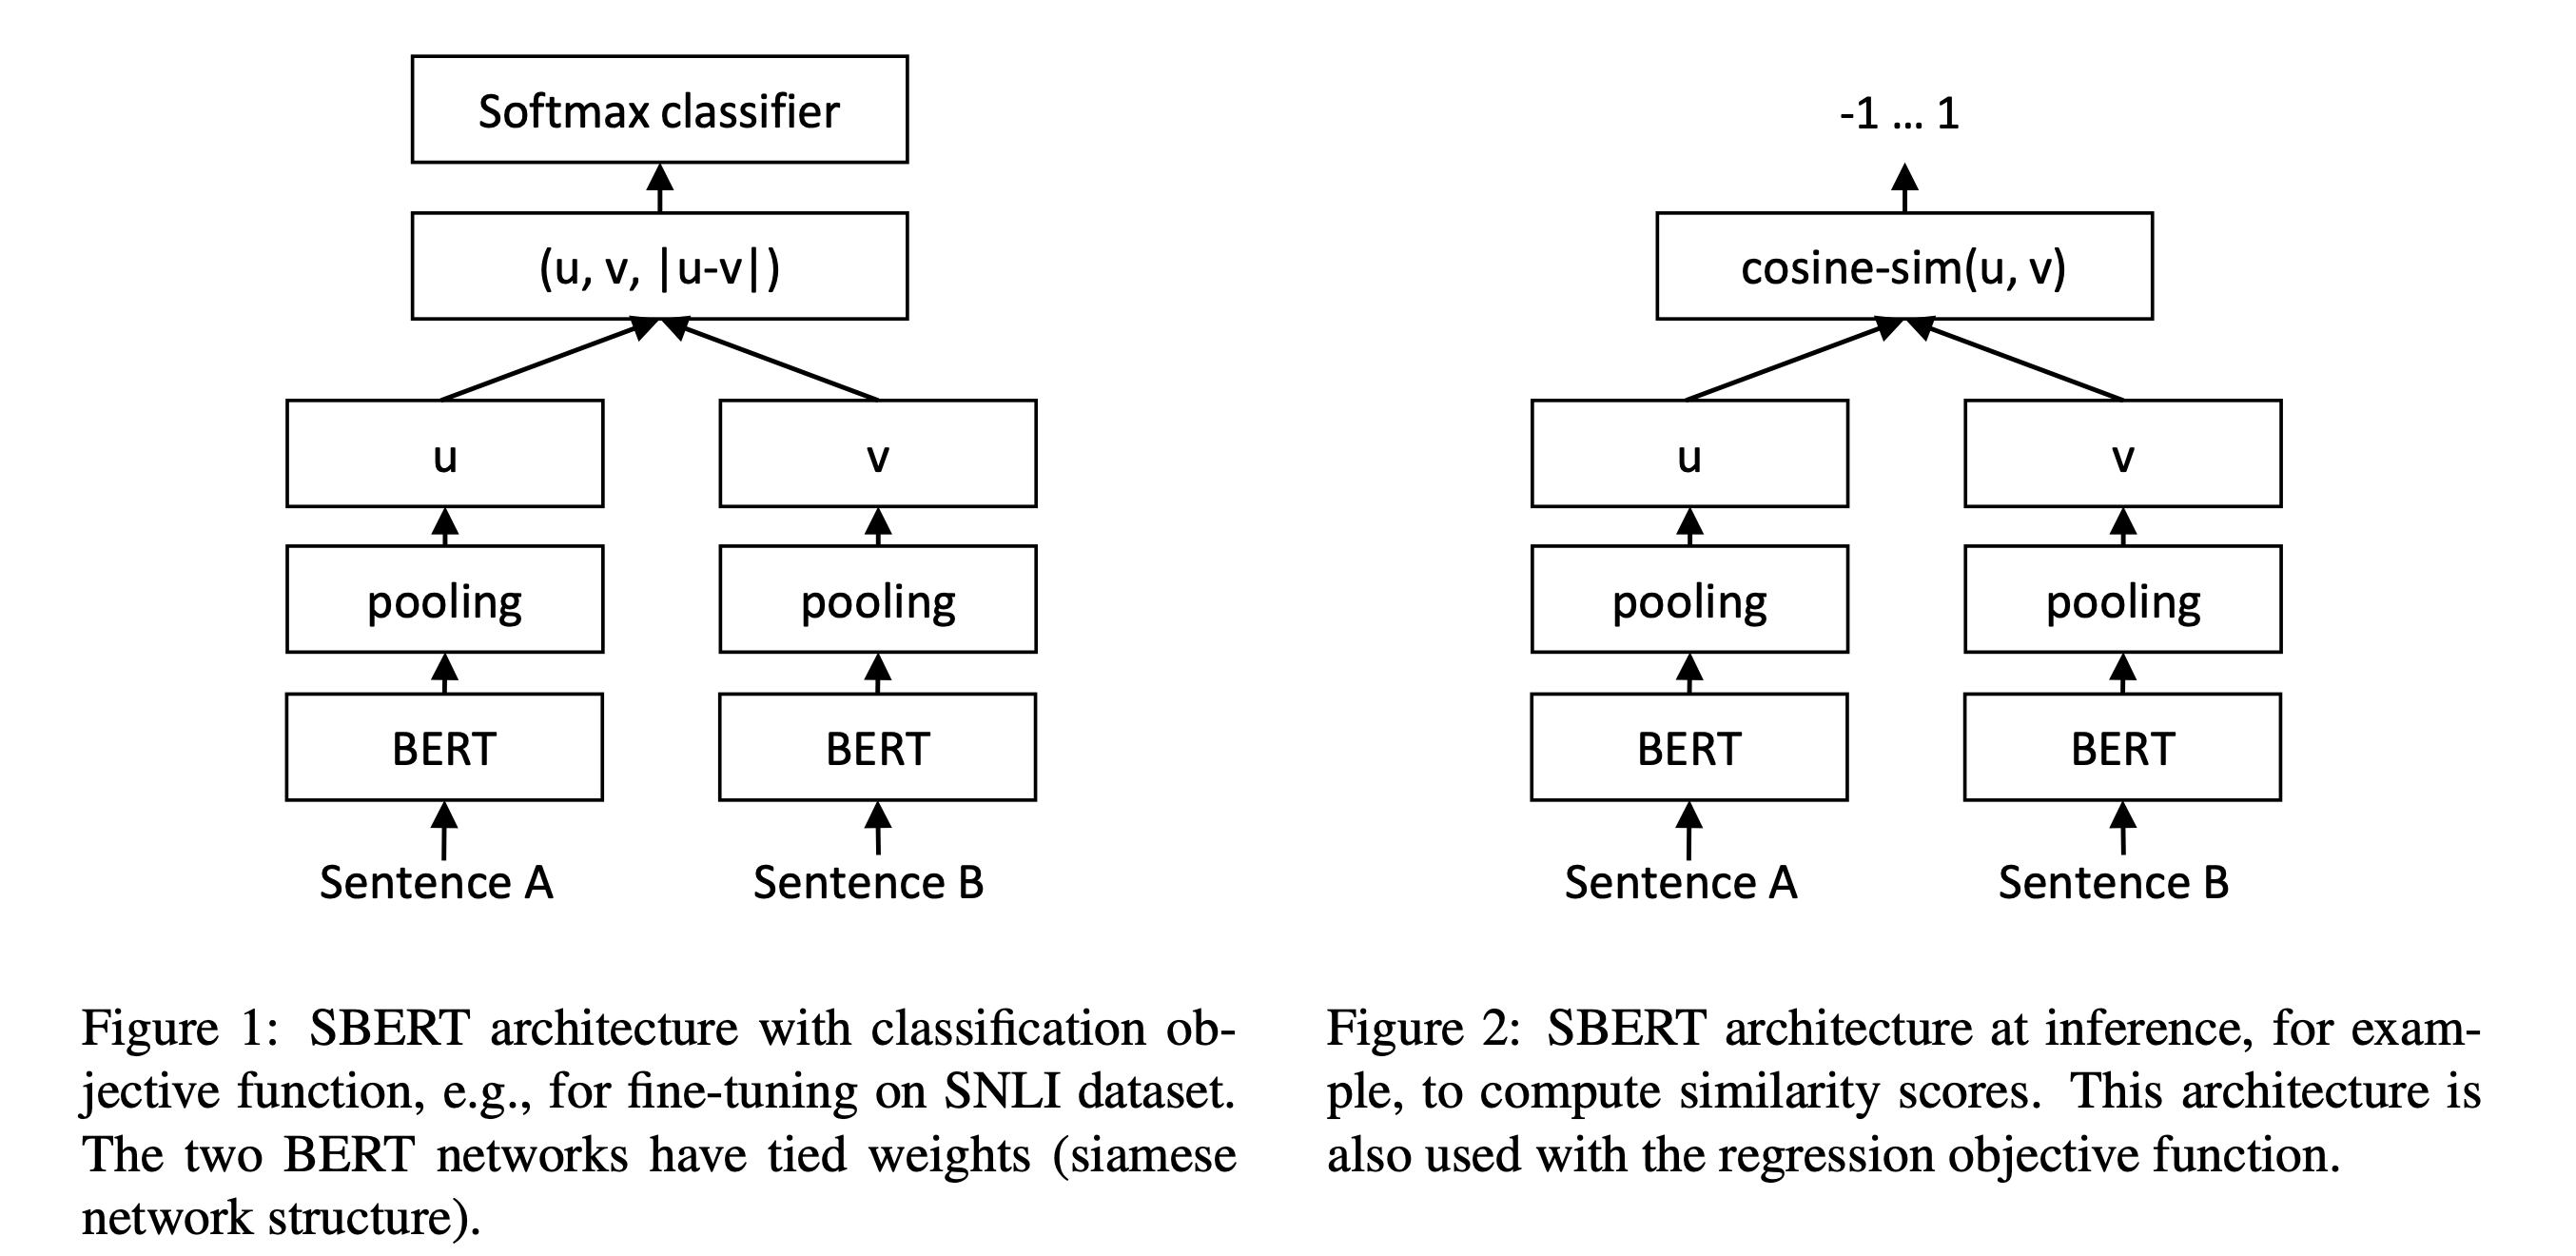
\includegraphics[width=1\linewidth]{Images/sentence_transformer.png}
    \caption{Sentence Transformer Architecture explained in\cite{reimers2019sentencebertsentenceembeddingsusing}}
    \label{fig:placeholder}
\end{figure}
Since BERT outputs contextual embeddings for individual tokens, an additional pooling layer is required to derive a single sentence vector, as shown in Figure~\ref{fig:Sentence_embedding}. In \cite{reimers2019sentencebertsentenceembeddingsusing}, the preferred pooling method for \glsxtrfull{STS} tasks is mean pooling, which turns multiple token embeddings into a single sentence embedding.\footnote{Other pooling strategies, such as using the \texttt{[CLS]} token or max pooling, were also evaluated but performed worse for semantic similarity tasks.}

\begin{figure}[h!]
    \centering
    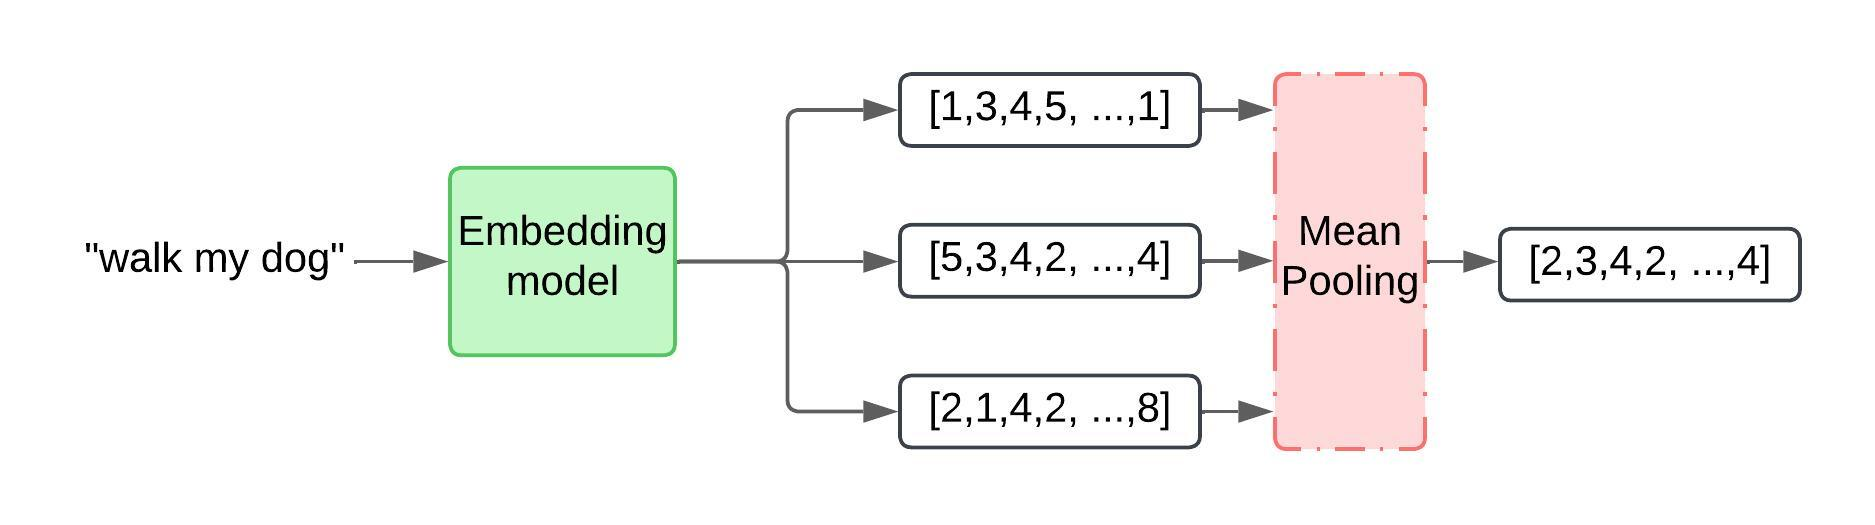
\includegraphics[width=1\linewidth]{Figures/Sentence_Embedding.jpeg}
    \caption{Example illustration of sentence embedding through mean pooling.}
    \label{fig:Sentence_embedding}
\end{figure}

To ensure that these embeddings capture sentence-level meaning, SBERT is fine-tuned on tasks such as Natural Language Inference (NLI), Semantic Textual Similarity (STS), and triplet training. 

When trained on NLI data with a classification objective, SBERT further compares pairs of sentence embeddings by constructing a combined feature vector $(u, v, |u-v|)$, where $u$ and $v$ are the pooled embeddings of the two sentences. This representation proved effective in downstream tasks such as the Semantic Textual Similarity benchmark (STS-b).

The quality of a Sentence Transformer is ultimately reflected in the accuracy and robustness of the embeddings it produces. Recent research has extended these methods to Portuguese, with the current state-of-the-art being the \textit{Serafim 900M IR} model \cite{gomes2024opensentenceembeddingsportuguese}, which has been specifically trained and benchmarked for \glsxtrfull{STS} and \glsxtrfull{IR} tasks.

\section{Vector Databases}
\label{sec:vector-store}
As described in more detail Section~\ref{sec:Sentence-Transformers}, embedding models transform unstructured data (e.g., text, images, or audio) into high-dimensional numerical vectors that capture semantic relationships. In such a vector space, similar objects are positioned closer together, while unrelated ones are placed farther apart. For example, the terms \emph{dog} and \emph{wolf} would be embedded near each other, whereas \emph{banana} would appear in a distant region (see Fig.~\ref{fig:vector-embedding}).  

A vector database stores these embeddings and supports efficient similarity search through vector indexing techniques, enabling similarity search at scale.
\begin{figure}[h]
    \centering
    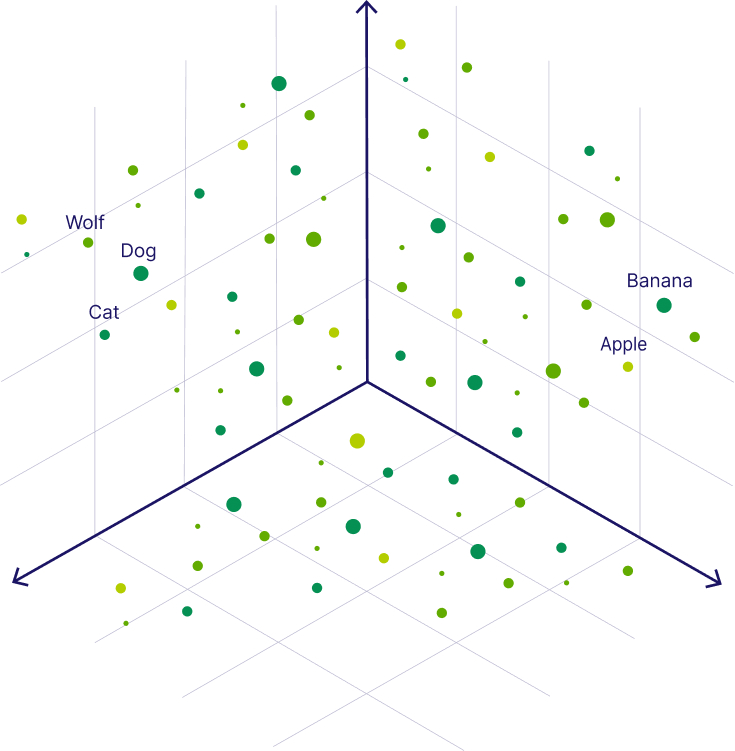
\includegraphics[width=0.55\linewidth]{Images/vector-embedding.jpg}
    \caption{Example of vector embeddings where semantically related terms are placed closer in the vector space \cite{weaviate}}
    \label{fig:vector-embedding}
\end{figure}

During inference, vector databases enable fast retrieval of relevant embeddings using Approximate Nearest Neighbor (\glsxtrfull{ANN}) search. 
Indexing algorithms such as \glsxtrfull{HNSW}, IVF, Product Quantization (PQ), or ANNOY are commonly employed. 
These methods differ in how they organize the search space: 
\glsxtrfull{HNSW} constructs a hierarchical graph, which supports dynamic insertion of new vectors and logarithmic-time search, making it suitable for continuously growing datasets. 
ANNOY (Approximate Nearest Neighbors Oh Yeah) builds static random-projection trees that are optimized for read-heavy workloads, but generally require index rebuilding when new vectors are added. 
IVF (Inverted File Index) partitions the vector space into clusters and restricts search to the most relevant clusters, which reduces query time at the cost of some recall. 
PQ (Product Quantization) compresses vectors into smaller codewords, drastically reducing memory consumption while enabling efficient approximate similarity computations. 

Figure~\ref{fig:semantic-search-pipeline} illustrates the flow from raw data to evaluation: embeddings are indexed using ANN algorithms and queried using a vector representation of the input. The retrieved results are then evaluated using similarity metrics \ref{sec:vector-similarity}
\begin{figure}[H]
    \centering
    \begin{tikzpicture}[
        node distance=1.7cm and 2.2cm,
        every node/.style={font=\small, align=center},
        process/.style={rectangle, draw=black, rounded corners, minimum height=1.1cm, minimum width=2.8cm},
        arrow/.style={->, thick}
    ]
        % Nodes
        \node[process] (input) {Unstructured Data \\ (Text, Image, Audio)};
        \node[process, right=of input] (embed) {Embedding Model \\ (e.g., SBERT)};
        \node[process, right=of embed] (index) {Vector Database \\ + ANN Index (e.g., HNSW)};
        \node[process, below=of index] (query) {Query Embedding};
        \node[process, left=of query] (retrieval) {Nearest Neighbors \\ (Top-K Retrieval)};
        \node[process, below=of retrieval] (metrics) {Similarity Metrics \\ (Cosine, Dot, Euclidean)};

        % Arrows
        \draw[arrow] (input) -- (embed);
        \draw[arrow] (embed) -- (index);
        \draw[arrow] (query) -- (index);
        \draw[arrow] (index) -- (retrieval);
        \draw[arrow] (retrieval) -- (metrics);
    \end{tikzpicture}
    \caption{Semantic retrieval pipeline: data is embedded, indexed, and queried using vector similarity search. Retrieved vectors are then evaluated using similarity metrics.}
    \label{fig:semantic-search-pipeline}
\end{figure}

\subsection{HNSW: Hierarchical Navigable Small World Graph}

\glsxtrfull{HNSW}~\cite{malkov2018efficient} is a graph-based indexing algorithm widely used in vector databases for approximate nearest neighbor (\glsxtrfull{ANN}) search. It is based on the principle of small-world networks, where most nodes can be reached in a small number of steps, despite the overall network being large.

\begin{itemize}
    \item \textbf{Graph Construction.} HNSW builds a multi-layer graph where each layer is a proximity graph: nodes (vectors) are connected to their closest neighbors according to a similarity metric (e.g., cosine similarity or Euclidean distance). The top layers have fewer nodes and longer links, forming a hierarchical structure. New vectors are inserted from the top layer down to the bottom, gradually establishing local connections at each level.

    \item \textbf{Search Process.} The search begins at the topmost layer and navigates greedily toward the query vector by moving to the closest neighbor at each step. Once a local minimum is reached, the process descends to the next layer and repeats, refining the search as it approaches the bottom layer (the densest one). The final result is a list of approximate nearest neighbors from the base layer.

    \item \textbf{Time and Space Complexity.} HNSW offers logarithmic search complexity—$\mathcal{O}(\log N)$ in practice—and supports dynamic insertion of vectors, unlike many tree-based or clustering-based methods. It requires additional memory for storing the graph structure, but in return provides excellent trade-offs between recall, latency, and update support.
\end{itemize}

Compared to other indexing methods such as IVF or ANNOY, HNSW tends to achieve higher recall at lower latency, especially in scenarios where index updates are frequent or low-latency responses are critical. Due to these properties, HNSW is the default index used in several vector databases such as FAISS, Milvus, and Weaviate.

\subsection{Vector Similarity}
\ref{sec:vector-similarity}
The similarity between vectors can be computed using several distance or similarity metrics, which are also employed in later semantic evaluation tasks with metrics such as:

\begin{itemize}
    \item \textbf{Cosine similarity:} computes the cosine of the angle between two vectors. It is invariant to magnitude, making it useful when semantic meaning is encoded in direction rather than length:  
    \[
        \textit{cos\_sim}(\mathbf{u}, \mathbf{v}) = \frac{\mathbf{u} \cdot \mathbf{v}}{\|\mathbf{u}\| \, \|\mathbf{v}\|}
    \]
    
    \item \textbf{Euclidean distance:} computes the straight-line distance between two vectors in the embedding space. It is effective when similarity correlates with geometric closeness:  
    \[
        d_{\textit{euclidean}}(\mathbf{u}, \mathbf{v}) = \|\mathbf{u} - \mathbf{v}\|_2 = \sqrt{\sum_{i=1}^n (u_i - v_i)^2}
    \]
    
    \item \textbf{Dot product:} measures the projection of one vector onto another, capturing both direction and magnitude. It is frequently employed in large-scale retrieval systems to approximate inner products between compressed vectors:  
    \[
        \textit{dot}(\mathbf{u}, \mathbf{v}) = \sum_{i=1}^n u_i v_i
    \]
\end{itemize}


Vector databases exist across a spectrum of complexity. Full-featured systems such as Weaviate, Pinecone, and Milvus provide distributed storage, hybrid queries, and built-in integrations with embedding providers.

\section{Text Similarity metrics}
Since this thesis aims to enhance semantic search through Retrieval-Augmented Generation (\glsxtrfull{RAG}), 
evaluating similarity between texts becomes a critical component for evaluating the model and methodology. 
No single metric fully captures the notion of similarity: some emphasize exact lexical overlap, 
while others account for structural variation or semantic equivalence. 
Therefore, a diverse set of metrics is employed to provide a more comprehensive assessment, 
ensuring that evaluation reflects the multifaceted nature of semantic search.

\subsection{Evaluation Metrics}

Since this thesis focuses on enhancing semantic search through \glsxtrfull{RAG}, the evaluation of similarity between retrieved passages, generated answers, and gold references is a critical step in evaluation. Different metrics capture complementary aspects of similarity, ranging from exact lexical overlap to semantic equivalence. Using a diverse set of metrics ensures that evaluation does not rely on a single definition of similarity, but instead reflects the multifaceted nature of semantic search.
\subsubsection{Binary Matching}
Exact match and substring match are both binary identification methods. Exact Match, checks if both texts are exacly the same. While substring match check if the gold reference is in the answer. These metrics are fast and simple, but are very lexically strict.

\subsubsection{Token Recall} 
Token Recall measures the proportion of reference tokens covered by the prediction:
\[
\text{Recall} = \frac{|A \cap G|}{|G|}
\]
where \(A\) and \(G\) denote the token sets of the answer and reference.  

\subsubsection{Jaccard Similarity} 
Introduced by Jaccard \cite{jaccard1901distribution}, this metric is defined as
\[
J(A,B) = \frac{|A \cap B|}{|A \cup B|}
\]
with \(A\) and \(B\) as token sets.  

\subsubsection{Levenshtein Similarity} 
Based on the edit distance proposed by Levenshtein \cite{levenshtein1966binary}, it is given by
\[
1 - \frac{\text{ED}(A,B)}{\max(|A|,|B|)}
\]
where \(\text{ED}\) is the edit distance between token sequences.  
\footnote{Edit distance is defined as the minimum number of operations (insertions, deletions, or substitutions of tokens) required to transform one sequence into the other.(e.g., transforming “cat sat” into “the cat” requires one insertion and one deletion)}

\subsubsection{ROUGE-n} 
Introduced by Lin \cite{lin2004rouge}, ROUGE measures n-gram overlap between candidate and reference. 
\footnote{An \emph{n-gram} is a contiguous sequence of \(n\) tokens from a text; for example, for the sentence ``the cat sat'', the unigrams (\(n=1\)) are {the, cat, sat}, while the bigrams (\(n=2\)) are {the cat, cat sat}.
ROUGE-1 therefore evaluates unigram overlap, while ROUGE-2 evaluates bigram overlap, which captures short phrase structure in addition to individual words. }
For n-grams of size \(n\), the metric is defined as:
\[
\text{Precision} = \frac{\text{overlap}}{\text{n-grams}(A)}, \quad
\text{Recall} = \frac{\text{overlap}}{\text{n-grams}(B)}, \quad
F1 = \frac{2PR}{P+R}
\]

\subsubsection{BERT-based Cosine Similarity.} 
This metric employs dense sentence embeddings from \textit{SentenceTransformer all-MiniLM-L6-v2} \cite{reimers2019sentence}. 
Similarity is computed as cosine similarity:
\[
\cos(\theta) = \frac{v \cdot u}{\|v\| \, \|u\|}
\]

\subsubsection{Overlap Coefficient.} 
Also known as the Szymkiewicz--Simpson coefficient \cite{simpson1960similarity}, it is defined as
\[
\text{Overlap}(A,B) = \frac{|A \cap B|}{\min(|A|,|B|)}
\]

\subsubsection{BLEU.} 
Introduced by Papineni et al. \cite{papineni2002bleu}, BLEU computes modified n-gram precision with a brevity penalty:
\[
\text{BLEU} = \text{BP} \cdot \exp\left(\sum_{n=1}^{N} w_n \log p_n\right)
\]
where \(p_n\) are modified n-gram precisions, \(w_n\) are weights, and BP is the brevity penalty.

By combining these metrics, the evaluation captures complementary perspectives:  
lexical accuracy (Exact Match, Substring, Jaccard), structural similarity (Levenshtein, ROUGE, BLEU), coverage of reference information (Token Recall, Overlap coefficient), and semantic equivalence (BERT cosine).This multidimensional evaluation approach allows for a comprehensive assessment by testing both surface-level metrics and deeper semantic understanding.

\section{Key Takeaways}
This chapter established the foundations of retrieval in modern intelligent systems. Machine learning models based on BERT-transformer \cite{bertpretrainingdeepbidirectional} arquitecture and variants surpass purely lexical methods by providing semantic understanding. Vector databases store their embeddings in efficient indexes for nearest neighbor search, enabling efficient retrieval tasks such as question answering. Similarity metrics complete the foundation by offering tools to evaluate performance, forming the basis for later experimentation with prompt engineering.
%\subsection{Rag Variants}

%\=printf("\glsxtrfull{%s}", toupper(submatch(1)))rag} is a novel approach to \glsxtrfull{nlp} that aims to improve the performance of \acpl{llm} on knowledge-intensive tasks. \glsxtrfull{rag} overcomes limitations of existing \acpl{llm} by combining a pre-trained sequence-to-sequence (seq2seq)  model (parametric memory) with a dense vector index to a vector database acessed via a neural retriever (non-parametric memory). Parametric memory, comes from the generator component \glsxtrfull{llm} itself. the non-parametric memory is part of the retrieval component,  based on a bi-encoder architecture. A document encoder produces a dense representaion of a document, and a query encoder produces a representation of the input query. The retriever is initialized using a pre-trained bi-encoder that has been trained to retrieve documents containing answers to questions. There reason why it is important to differentiate parametric memory with non-parametric memory is that they have some key differences. Non-parametric memory for can be easily updated by replacing the document index, is also more interpretable because it consists of raw text that is human readable, 

%What is \acentrylong{rag} and why is it so important in organizations.\=printf("\glsxtrfull{%s}", toupper(submatch(1)))llm} have shown that they are able to store factual knowledge in their parameters. And by themselves can give information. The problem is that to add information to it, the model must be trained again. Also the model can give you information, but will not provide the source of information. So the information cannot be verified, and so it cannot be used in a corporate environment, as \glsxtrfull{llm} can also hallucinate knowledge.

%\section{Access Control Lists}

% #############################################################################





